
\documentclass[conference]{IEEEtran}

\usepackage[dvips]{graphicx}
  % declare the path(s) where your graphic files are
\graphicspath{{images/}}
  
\usepackage{algorithmicx}

\hyphenation{op-tical net-works semi-conduc-tor}


\begin{document}
%
% paper title
% can use linebreaks \\ within to get better formatting as desired
\title{Society News Detection System}


% author names and affiliations
% use a multiple column layout for up to three different
% affiliations
\author{\IEEEauthorblockN{Chen Jie}
\IEEEauthorblockA{School of Computer Science\\
Beijing Institute of technology\\
Beijing, Haidian district\\
Email: sonyfe25cp@gmail.com}
\and
\IEEEauthorblockN{Zhendong Niu}
\IEEEauthorblockA{School of Computer Science\\
Beijing Institute of technology\\
Beijing, Haidian district\\
zniu@bit.edu.cn}
\and
\IEEEauthorblockN{Yulong Shi\\ and Changmin Zhang}
\IEEEauthorblockA{School of Computer Science\\
Beijing Institute of technology\\
Beijing, Haidian district\\
}
}


\maketitle


\begin{abstract}
%\boldmath
Since so many news media ouput huge volume web news, it's hard for people to know how many events happened everyday and how is the progress of some event . In this paper, we report a society news event detection system ,which help people to get the lastest event occured. The system contains three parts: society news qcquisition module , event detection module and event summariation module.
\end{abstract}

\IEEEpeerreviewmaketitle

\section{Introduction}
% no \IEEEPARstart
With the rapid progress of technologies for information dissemination, more and more people choose Internet media instead of traditional ones as their main way to get fresh information. As a result, online news platform, one of the most important network information forms, gets a rapid growth during the past few years. Most of the popular websites have their own online news platform to attract more visitors since it is fast and real-time to get the latest trends. However, preciously because of the rapid expansion of online news, it is more and more difficult to find out valuable information from such large scale data. Especially when we want to know the development of some special events quickly, we must spend time searching and filtering out noises to get what we want by ourselves which leads a bad user experience. Event detection system which can gather relevant news and reports describing the same event automatically comes into being in such a case.

Event is a series of activities occurring at specific time and specific place, involving specific subjects and along with some consequences. It normally consists of news and reports with the same topic and has the following features. Firstly, all of these news and reports have a same topic, namely, they all describe a same event. Secondly, these reports reflect the development and latest trends of an event. For example, reports about the eruption of earthquake in Yaan and the following series of news about casualties and rescues all belong to the same event. Thirdly, all relevant reports should be included in the event.

In this paper, we design an event detection system based on J2EE aiming at providing an efficient service to users. Our system can extract news from popular news websites, aggregate all the relevant news describing the same event together automatically and display them in event forms. It is easy for users to scan and get a global picture about an event which is time saving and has a very high practical value. And also, our system can detect the newest report about the current event and add it to the news set in near real time which is a new feature of our system compared to those old ones.

The remainder of this paper is organized as follows: Section 2 reviews some related works on event detecting system. We discuss the framework, functions and some techniques used in our system in Section 3. Our experiments and the analysis of the results are described in Section 4. Section 5 presents our future plans.

% You must have at least 2 lines in the paragraph with the drop letter
% (should never be an issue)
%I wish you the best of success.

\section{Related works}

Event discovery is one practical application of the technique of topic detection and tracking. At present, most of the event detection systems are completed based on document cluster and vector space model (VSM) technologies and researchers have came up with a series of algorithms and methodologies, such as hierarchical clustering, single-pass clustering, incremental K-medoids clustering, etc.

D.Trieschnigg\cite{2005-Trieschnigg-p55-62} put forward a scalable hierarchical theme detection model. Unlike\cite{2007-Pons-Porrata-p752-768}, A.P.Porrata et al. came up with an improved incremental hierarchical clustering algorithm to detect topics by combining classification and hierarchical clustering technologies. Huang et al. \cite{2011-Huang-p280-284} put forward a novel news event detection method by using named entity when clustering. Yang \cite{2010-Yang-p372-374} analyzed the characteristics of social network such as microblog and BBS, and came up with an approach of detecting news event from noisy textual datasets. Besides text itself, we can also use other information to improve the detection probability when detecting events from news stream. Sun et al. \cite{2011-Sun-p834-839} suggested a query-guided news event detection method by analyzing user’s query, news’ title and content. Dai et al. \cite{2010-Dai-p3341-3346} thought that terms located at different areas have different distributions to similarity. For example, terms in title should make greater contribution than those in body. Based on the theory, Dai et al. put forward an improved hierarchical clustering algorithm to detect topics and an improved single-pass clustering method to track topics.

Discovering new event, the task of which is to decide which event we should locate a new report to, is one of the important modules of event detection technique. Papka et al.\cite{1998-Papka-p-} put forward a single-pass clustering approach. Firstly, they preprocessed a new coming news report and converted it to weighted vectors. Then, they calculated the similarities between the new coming news report and each of the existing records. Finally, they defined the new coming news to a new event if all of the similarities are less than the threshold. Lam et al. \cite{2001-Lam-p525-546} compared the similarities between the new coming report and all the detected events. Then they allocated the report to the cluster which has the largest similarity with it if the similarity is larger than the threshold. Otherwise, they defined a new event to hold the new coming report. Jia et al. \cite{2004-JIA-p32-32} put forward an algorithm based on dynamic evolution model to detect and track news event by combining single-pass clustering and news characteristics. 

In this paper, we design a news event detection system based on J2EE techniques. Firstly, we crawl news web pages from some popular websites using web crawlers and extract content from these web pages. Secondly, we calculate the similarities between these news reports. Thirdly, we use undirected graph to cluster the web pages with the same topic together to generate the corresponding events.

\section{System Architecture and Function Design}
In this chapter, we firstly introduce our system architecture and work flow briefly. And then we will discuss the key functional modules and key techniques we used in detail.
\subsection{System Framework}
Our system is based on J2EE framework and has 4 main modules: news crawling, content extracting, similarity computing and event discovering. And all the three former ones are the preparation stages of the last one. The work flow is as follows: Firstly, crawl all the news web pages from specified websites using web crawlers and save them as texts. Secondly, parse web pages and filter out the irrelevant factors (html tags, etc) as well as extract structure information, such as title, body, author and so on. Thirdly, build inverted index for the filtered news text according to the structure. Fourthly, compute the similarities of news texts by analyzing the index information established at step 3. Lastly, cluster news reports to corresponding events according to the similarities. Figure ~\ref{fig:systemprocess} shows the relationship of these system modules and the work flow of the whole system.

\begin{figure}
\centering
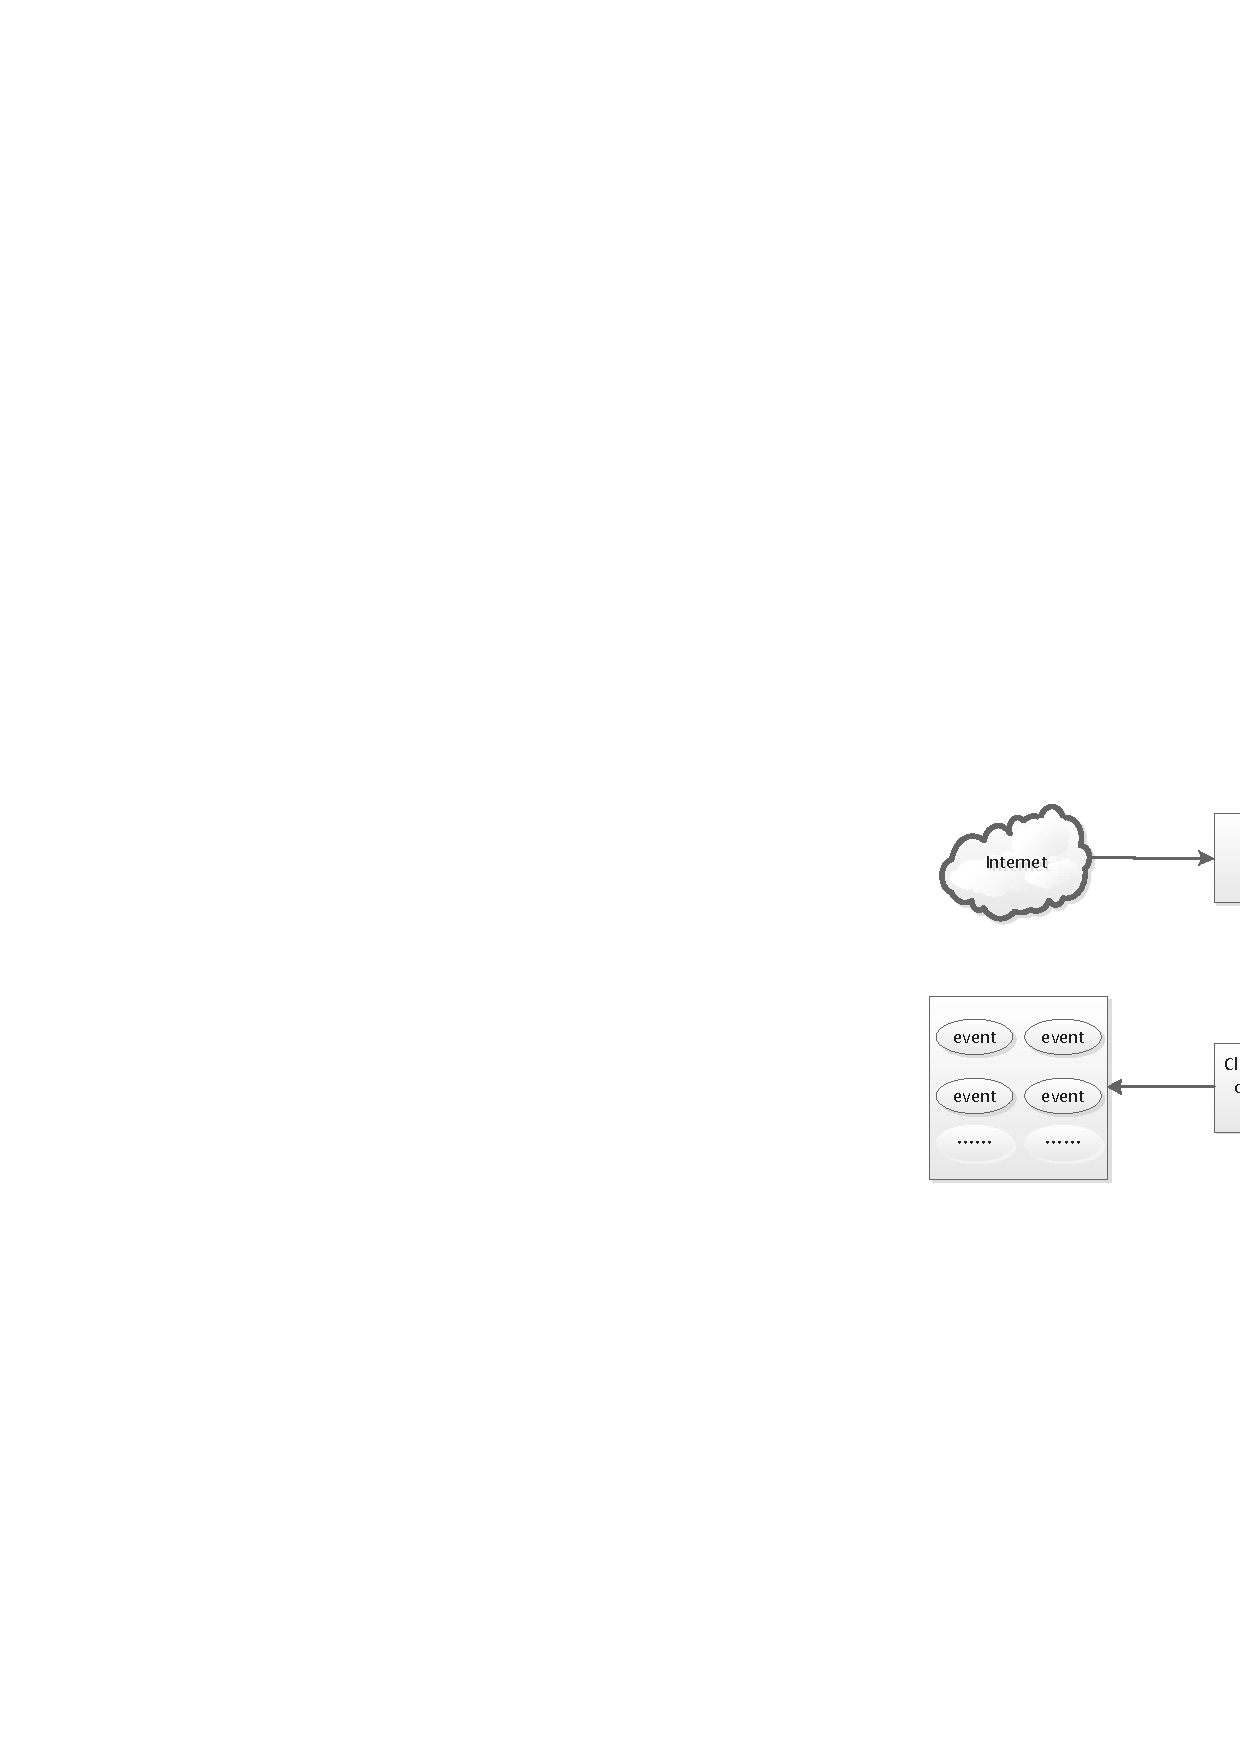
\includegraphics[width=2.5in]{process}
\caption{The process of this society news detection system}
\label{systemprocess}
\end{figure}

\subsection{Topic web crawler on society news}

Topic web crawler constitutes the news acquistion module. It's the data source of this system and determines whether the contents of the entire wealth of information systems as well as timely news updates. The principle of a web crawler is descriped in  Fig \ref{fig:crawler}. Firstly, crawler will get the souce code of web pages based on the initial URL seeds.Secondly,  after parsing the URL from these pages, the crawler will remove all the URLs that already crawled and put new coming URLs into the queue. Thirdly, the crawler will do this loop untils the queue is empty or some specific stop condition reached. 
\begin{figure}
\centering
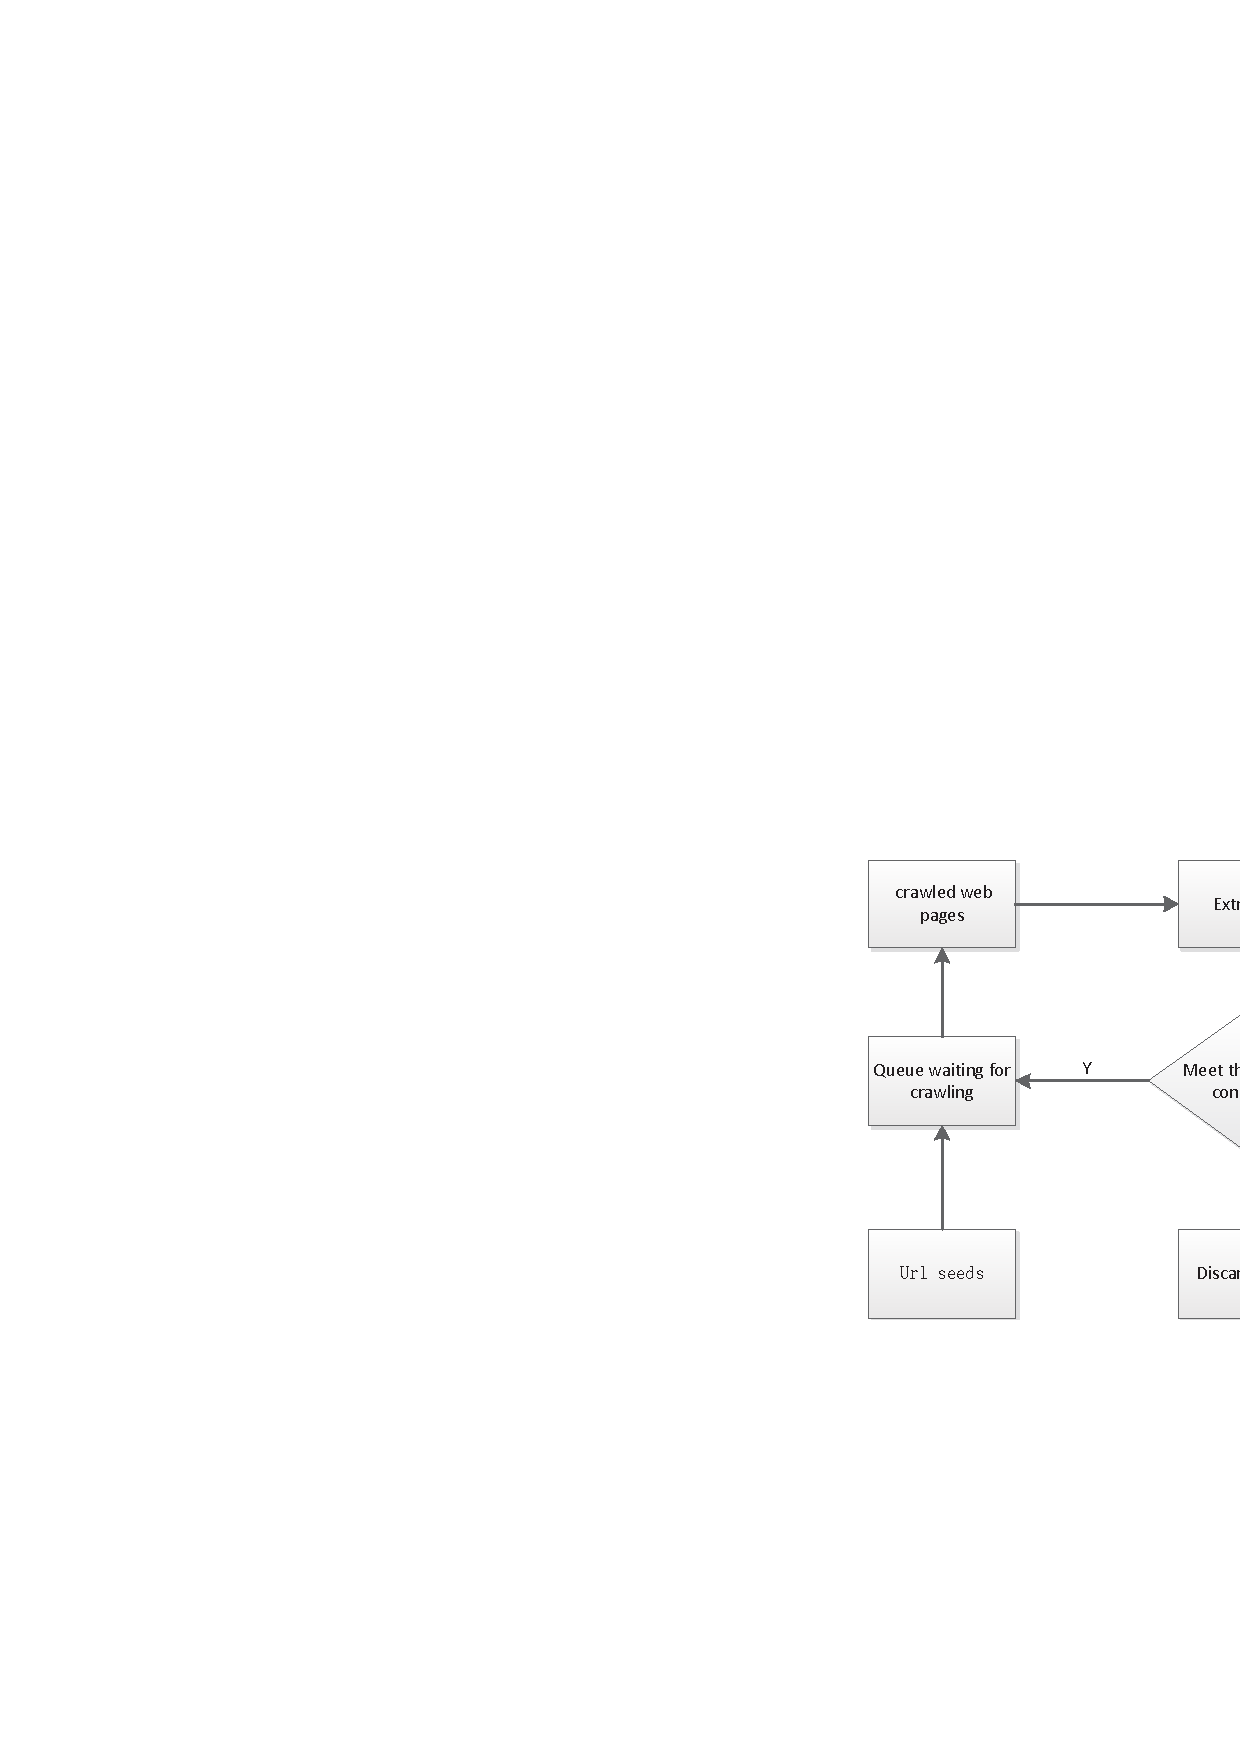
\includegraphics[height=2.5in]{crawler}
\caption{the principle of web crawler}
\label{fig:crawler}
\end{figure}
The goal of society news topic web crawler is to do classification to the pages , store the news belong to society news and remove others. We get the train data from some big news media website, crawl pages from different channels and labeled them as their channel. For example, we label the news from sports channel to sport class. With this kind of training data, we train a classificator based on native bayes algorithm.Firstly, we cut the sentence into words with word parser and  remove stop words and . Secondly ,  we count the occurrence number of each word group by labels. Thirdly, we can compute  whether the new comming pages belong to the society news group by fomular \ref{nativebayes}
\begin{equation}
P(C_i|X) = \frac{P(X|C_i) P(C_i)}{P(X)}
\end{equation}
\begin{equation}
P(X|C_i) = \prod_{k=1}^n P(X_k|C_i) = P(x_1|C_i) * P(x_2|C_i)* \dots * P(x_n|C_i)
\end{equation}


\subsection{Web content parsing}

As the web pages crawled by web crawler contain much irrelevant information, like html tags, javascript and so on, we need preprocess the data before using it, which consists of two steps: content extraction and inverse index establishment.

A combination of a segmentation-like approach and a density-based approach  are used to extract the main content  of web page[7]. Firstly, we construct a DOM tree for the original web pages. And then convert the DOM tree to more easily processed BLE\&IE blocks. BLE are defined that elements displayed as block margins in a new line with independent height and width. They can only contain text or IE.A BLE\&IE block is a labeled ordered tree that is converted from a node tree by some specific operations. The root of a BLE\&IE block is a BLE. A regular expression , $(IE|text)*p?q*|l*|t*$, used to match the blocker from the source code .

After converting the DOM to BLE\&IE blocks, we process them with a density-based content extract algorithm to distinct the content from noisy data. The density of a node or a BLE\&IE block is the ratio of TextLength to TagLength. And the ratio is based on such a fact that in HTML documents, contents always contain large numbers of characters and need comparatively fewer characters to describe their tags, while texts in noises always contain small numbers of characters and need comparatively more characters to describe their tags. And only the nodes with higher densities than threshold can be regarded as candidate content. The procedure of the above description can be expressed as follows:
\begin{algorithm}
\end{algorithm}

\subsection{Society events detection}
According to the definition of event, a series of news stories having a same or similar topic can be called an event. 
The goal of society events detection is that cluster the big volumn society news into different events.  The detection of event divide in two steps: news representation and event detection.

\subsubsection{News representation and similiarty matric}

We express each news text with a vector, and each element in vector presents the weight of term t in document d. Here we compute the weight with TFIDF, which is showed as below:
\begin{equation}
w(t,d) = \frac{d_t}{|d|} * log(\frac{N+0.5}{N_t=1})
\end{equation}
Where $d_t$ means the frequency of term $t$ in document $d$, $| d|$ is the number of terms document $d$ contains, $N_t$ is the number of documents that contain term $t$, $N$ is the number of documents in the corpus.
Then we compute the similarity of two documents using the expression below:
\begin{equation}
Sim(d_i, d_j) =  \frac{\sum_{t \in (d_i \bigcap d_j)}w(t,d_i)*w(t,d_j)}{\sqrt{\sum_{t \in d_j} w(t,d_i)^2 } * \sqrt{\sum_{t \in d_j} w(t,d_j)^2}}
\end{equation}

\subsubsection{event detection}
With the expression above, we can obtain the similarity between any two documents and generate the similarity matrix. Then we can utilize the undirected graph to discover news reports with the same topic and cluster them together. In the undirected graph, each node presents a document. If there is an edge between two nodes, we say that the two documents have some relationship and the weight of the edge presents the similarity of the two documents. Here we defined a threshold parameter $\theta$, and connect two nodes with the weighted edge only when the similarity value is larger than the threshold. Finally, nodes at a same undirected graph consist of a news event, which can be showed as follows:

\subsection{Event summarization}
Our system also provides a functional module of automatic abstract for news event after the event discovery step so that users can get the useful information about the event more quickly. In our system, we extract sentences with a centroid-based method. Firstly, we use latent semantic analysis (LSA), a mathematical technique, to derive latent semantics from news. Secondly, we compute the distance between each sentence and the cluster centroid. Thirdly, the weight of each sentence can be obtained with a linear combination of the distance and the position where the sentence is located. Finally, we select the salient sentences with top weight and the minimum redundancy.

\subsubsection{Sematic analysis}

Here we use latent semantic analysis (LSA), a mathematical technique, to derive latent semantics from news. The process starts with the construction of a word-by-sentence matrix $A$, where each row indicates a word, each column indicates a sentence, and $a_{ij}$ indicates the weight of word $w_i$ in sentence $s_j$. Since every word does not normally appear in each sentence, the matrix $A$ is usually sparse. We then apply the singular value decomposition (SVD) to the matrix $A$, which is defined as:
\begin{equation}
A = U \Sigma V^T
\end{equation}
Where $U$ is an $m×n$ matrix whose columns are called left singular vectors, $\Sigma$ is an $n×n$ diagonal matrix whose diagonal elements are non-negative singular values sorted in descending order, and $V$ is an $n×n$ matrix whose columns are called right singular vectors.

Next, we perform a dimension reduction to the diagonal matrix $\Sigma$ by cutting down some elements in it and we get matrix $\Sigma '$. Then a new matrix $A'$ is reconstructed by multiplying three matrices as follows:
\begin{equation}
A'=U'\Sigma'V'^T \approx A
\end{equation}
Where $\Sigma$' represents the semantic space that can derive latent semantic structures from $A$, $U'$ and $V'$ is the dimension reduced matrices correspond to $U$ and $V$ respectively. Each column of $A'$ denotes the semantic sentence representation, and each row denotes the semantic word representation.

\subsubsection{Distance from the centroid}
A centroid is a set of words that are statistically important to a cluster of documents, which represents the core idea of an event. The closer with centroid, the more important information does the sentence contain. Here we use cosine similarity to express the distance between sentence and centroid. And the larger similarity value means the more important sentence.

Firstly, we generate the centroid of the cluster using the top K weighted words and phrases, which can be expressed as $S_c=(w_1,w_2,…,w_k)$. Then, we can calculate the similarities between each sentence and centroid and sort sentences by the similarity value descendingly.
\begin{equation}
W_D(S_i)  = Sim(S_i, S_c) =\frac{ \overrightarrow{S_i} \cdot \overrightarrow{S_c}  }{|S_i||S_c|}
\end{equation}
where $ \overrightarrow{S_i}$ is the vector of sentence $S_i$ and $\overrightarrow{S_c}$ is the vector of centroid $S_c$.

\subsubsection{Sentence Position}
Generally, sentences located at the head position contain more useful information than those at the tail position, so we should assign higher weight to former sentences. Here we simply compute the positional value of sentence by inverse the sentence position in document.
\begin{equation}
W_p(S_i) = \frac{1}{i}
\end{equation}

\subsubsection{Sentence Selection}
After the former steps, we can obtain sentence weight by linearly combining the centroid value and the positional value, which can be defined as follows:
\begin{equation}
W(S_i) = \lambda W_D(S_i) + (1- \lambda) W_p(S_i)
\end{equation}
Then the top N weighted sentences are selected as the candidate abstract sentences. 

\subsection{Experiments}

\subsubsection{Topic Web Crawler}


\subsubsection{Event detection}



\subsection{Conclusion}


\subsection{Subsection Heading Here}
Subsection text here.


\subsubsection{Subsubsection Heading Here}
Subsubsection text here.


\section*{Acknowledgment}


The authors would like to thank...



\begin{thebibliography}{1}

\bibitem{IEEEhowto:kopka}
H.~Kopka and P.~W. Daly, \emph{A Guide to \LaTeX}, 3rd~ed.\hskip 1em plus
  0.5em minus 0.4em\relax Harlow, England: Addison-Wesley, 1999.

\end{thebibliography}

\bibliographystyle{IEEEtran}
\bibliography{IEEEabrv,../../bib/news}


% that's all folks
\end{document}


